%! alt The octahedron with vertices (t, 0, 0), (0, t, 0), (0, 0, t) and their negatives, drawn for t = 5 in parallel projection with hidden edges dashed; the vertex (t, 0, 0) is at the front left. The face in the plane x + y + z = t and the opposite face in the plane x + y + z = -t are shaded. A line through the centre O in the direction (1, 2, 2) meets these two planes at X1 = (1, 2, 2) and X2 = (-1, -2, -2), and O is the midpoint of X1X2.
%! after_paragraph 1
%! scale 3/5
%! let a = 3/5
%! let b = 1/5
% The shared preamble of every Cevian figure. pipeline/figures turns these colours into theme-aware paint,
% and refuses any other colour, so draw only with them:
%   figink (lines and labels), figaux (construction lines), figaccent (the object the argument turns on),
%   figtint and figaccenttint (light fills).
\documentclass[border=1.5pt]{standalone}
\usepackage{tkz-euclide}
\definecolor{figink}{RGB}{0,0,0}
\definecolor{figaux}{RGB}{85,85,85}
\definecolor{figaccent}{RGB}{192,57,43}
\definecolor{figtint}{RGB}{221,221,221}
\definecolor{figaccenttint}{RGB}{245,213,208}
% tkz-euclide's defaults draw circles, compasses and marks in 50% grey and fill points with a tint.
\makeatletter
\def\tkz@otherlinecolor{figink}
\def\tkz@euc@circlecolor{figink}
\def\tkz@euc@compasscolor{figink}
\def\tkz@euc@mkcolor{figink}
\def\tkz@mk@fill{figink}
\def\tkz@euc@pointfillcolor{figink}
\makeatother
\tkzSetUpLine[color=figink,line width=.7pt]
\tkzSetUpArc[color=figink,line width=.7pt]
\tkzSetUpCompass[color=figink,line width=.5pt]
\tkzSetUpPoint[color=figink,fill=figink,size=3.1pt]
\tikzset{
  every picture/.style={line cap=round,line join=round,color=figink},
  circle style/.append style={color=figink,line width=.7pt},
  aux/.style={color=figaux,line width=.45pt,dash pattern=on 2.6pt off 2pt},
  key/.style={color=figaccent,line width=1pt},
  mk/.style={color=figink,line width=.5pt},
  lbl/.style={color=figink,inner sep=2.2pt},
  len/.style={color=figink,inner sep=1.5pt,font=\small},
}

\begin{document}
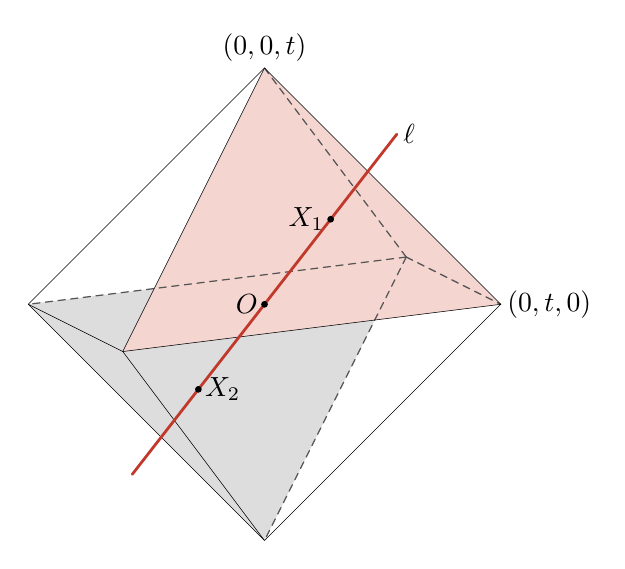
\begin{tikzpicture}
\tkzDefPoint(0.0,0.0){O} %! O = (0, 0)
\tkzDefPoint(-1.8000000,-0.60000000){Xp} %! Xp = (-5*a, -5*b)
\tkzDefPoint(1.8000000,0.60000000){Xm} %! Xm = (5*a, 5*b)
\tkzDefPoint(3.0000000,0.0){Yp} %! Yp = (5, 0)
\tkzDefPoint(-3.0000000,0.0){Ym} %! Ym = (-5, 0)
\tkzDefPoint(0.0,3.0000000){Zp} %! Zp = (0, 5)
\tkzDefPoint(0.0,-3.0000000){Zm} %! Zm = (0, -5)
\tkzDefPoint(0.84000000,1.0800000){Q} %! Q = (2 - a, 2 - b)
\tkzDefPoint(-0.84000000,-1.0800000){R} %! R = (-2 + a, -2 + b)
\tkzDefPoint(1.6800000,2.1600000){S} %! S = (2*(2 - a), 2*(2 - b))
\tkzDefPoint(-1.6800000,-2.1600000){T} %! T = (-2*(2 - a), -2*(2 - b))
%! fact collinear(Q, O, R)
%! fact collinear(S, O, T)
%! fact midpoint(O, Q, R)
%! fact parallel(Xp, Yp, Xm, Ym)
%! fact parallel(Yp, Zp, Ym, Zm)
%! fact parallel(Zp, Xp, Zm, Xm)
%! example area(Xp, Yp, Q) + area(Yp, Zp, Q) + area(Zp, Xp, Q) == area(Xp, Yp, Zp)
%! example 5 * area(Xp, Yp, Q) == area(Xp, Yp, Zp) * 2
\tkzFillPolygon[color=figtint](Xm,Ym,Zm)
\tkzFillPolygon[color=figaccenttint](Xp,Yp,Zp)
\tkzDrawSegments[aux](Xm,Yp Xm,Ym Xm,Zp Xm,Zm)
\tkzDrawSegments(Xp,Yp Xp,Ym Xp,Zp Xp,Zm Yp,Zp Yp,Zm Ym,Zp Ym,Zm)
\tkzDrawSegment[key](T,S)
\tkzDrawPoints(O,Q,R)
\tkzLabelPoint[left,lbl](O){$O$}
\tkzLabelPoint[left,lbl](Q){$X_1$}
\tkzLabelPoint[right,lbl](R){$X_2$}
\tkzLabelPoint[right,lbl](S){$\ell$}
\tkzLabelPoint[above,lbl](Zp){$(0,0,t)$}
\tkzLabelPoint[right,lbl](Yp){$(0,t,0)$}
\end{tikzpicture}
\end{document}
